\section{Algorithm}
%
%----- why we need this section: what we offered is abstract and
%implementing it is not obvious
In this section, we present a detailed and practical implementation
strategy of the operational semantics presented in section \ref{sec:semantics},
where we introduced an abstract outline of our consistency
preservation technique. Here we realize our consistency management technique by equipping 
each replica with a \emph{cache}, that is guaranteed to
preserve the specified consistency level. This requires a seperation
between the effects that are local to the replica and effects that have
been entered the cache. 

The necessaty of using a cache on top of the replica  can be clearly noted 
in \visrule step in our core operational
semantics, where the set $V$ of effects
is present at the replica, however the system only shows the subset $V'$
to the operation. Note
that by \emph{maintaining} a consistent cache, the system is liberated from the
redundant task of generating a consistent subset of effects at each
operation execution.
The cache maintenance at each replica boils down to two tasks. First the
replica must decide if a newly arrived remote effect can enter the
cache or not, i.e. if its presence in the cache will violate the
contract or not.  Second, when the operations are submitted, the replica
must decide if they should proceed or should be blocked temporarily,
untill more effects become available in the cache.  Here we assume a
contract of the form  
$\psi = \forall (a,b). a \xrightarrow{R} b  \Rightarrow a
\xrightarrow{\visZ} b$ and a replica containg a local set $V$ and explain each task in more detail.

Let's first define the \emph{truncated relation}, as the relation derived by
removing the last element from a given relation: 
\begin{smathpar}
trunc (r_1;r_2;...;r_k) = r_1;r_2;...;r_{k-1}
\end{smathpar}
We now extend the above definition to the given contract, by replacing
$R$ with $trunc(R)$ and argue that an effect $\eff$ can only enter the consistent cache, if
its presence would not violate the truncated contract,
i.e. $\eff$'s dependency set $(trunc(R))_V^{-1}(\eff)$ is already
present in the cache. Now we consider two cases and explain the
replicas' behavior when an operation is submitted: 
\begin{enumerate}
\item $r_k = \soZ$: In this case, the replica makes sure that the
operation is blocked until effects from earlier operations from the same
session, are already present in the cache. This guarantees the presence
of the dependencies of the effect being created, accoring to the
\emph{original} contract. Note that in this case, the operation can
witness \emph{all} effects at the replica.
\item $r_k = \visZ$: In this case, operations are not blocked, however,
they should only witness the effects that are already present in the
cache. This guarantees the preservation of the original contract, which
puts a maximal bound on the set of effects to be made visible to an
operation.
\end{enumerate}
%
%--- The memoization technique to avoid redundent computations
%
\subsection{Degree of Dependency Presence}
In the above description of our consistency management tool, the notion
of \emph{presence of the depency set} is treated as a true/false
property, that is checked before allowing an effect to enter the cache.
However, as an astute reader might have noticed, a naive implementation
of this idea, could result in a poor performance. That is because
contracts in our specification language can be arbitrarily large and
might contain closures of relations, computing the inverse of which can
become very large. A naive implementation that drops all the computations
done for a failed dependency check of an effect, results in redunencies
the next time the same property is being validated 
and is not practically reasonable.

To address the mentioned difficulties, we introduce the \emph{Degree of
Dependency Presence (DDP)}, that extends the above binary property, by
marking effects with a
number, that represents how far the dependencies of an effect are
present
The DDP of an effect accoring to a relation $R=r_1;r_2;...;r_k$ and a
given set of local effects $V$ is defined as the length of the longest
ending subsequence of $R$, under which $V\cup \{\eff\}$ is
consistent for operations.
i.e. 
\begin{smathpar}
DDP_V(\eff) = m \iff (r_{k-1-m};...;r_{k-1})_V^{-1}(\eff)\subseteq V
\end{smathpar}
For example $DDP_V(\eff)=1$  means $\eff$ has just arrived to the
replica and no degree of its dependencies are checked yet, and
$DDP_V(\eff)=k$ means that all degrees of $\eff$'s dependencies are
present and it is safe now to add it to the cache.

This way, by periodically refreshing the $DDP$ of effects, the porcess
of moving the effects from the replica to the cache is recorded as the
new dependencies arrive, and as we will explain shortly, we can totally avoid 
computing closures of relations and also redundencies at replicas. 
Finally, note that (following the discussion in previous section) we require 
the dependencies to be looked for, in the replica and the cache
respectively, for the  waiting and non-waiting contracts.
i.e. in the case of waiting contracts  $DDP_{replica}$ 
should be computed and $DDP_{cache}$
for non-waiting contracts.




\subsection{Example}
\begin{figure}[t]
	\centering
	\setlength{\fboxsep}{6pt}%
	%\framebox[0.87\textwidth]{
	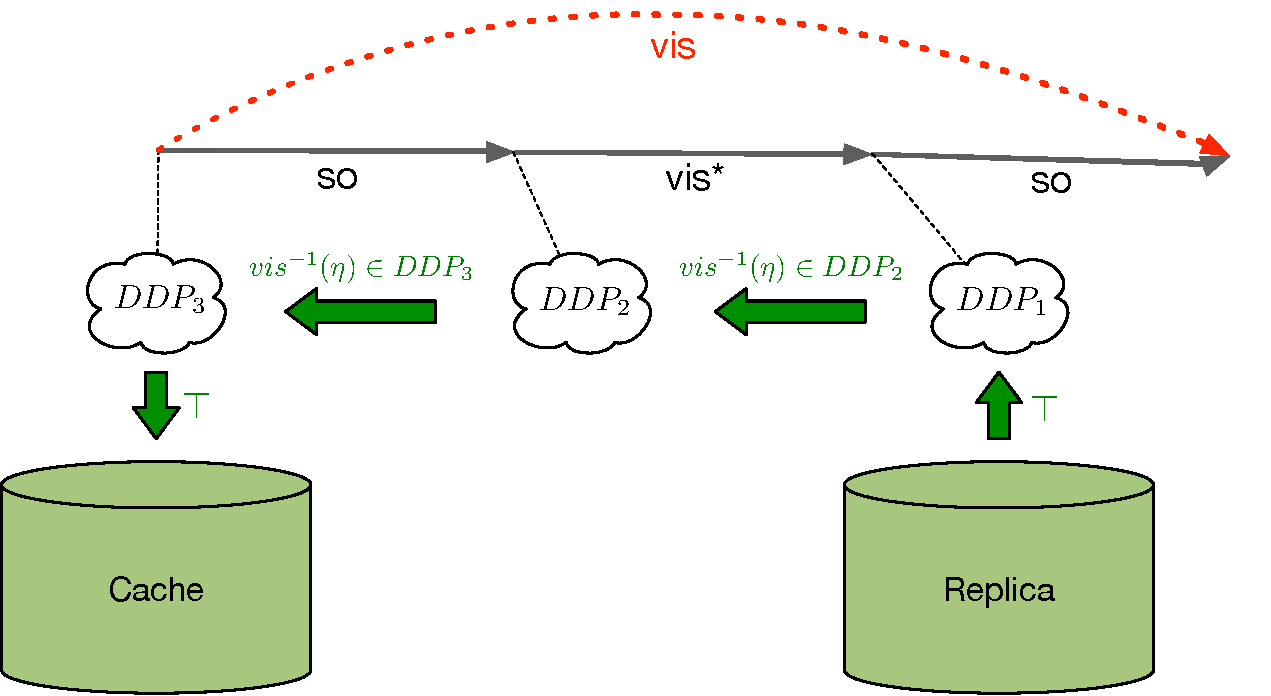
\includegraphics[scale =
	0.4]{Figures/Availability_deg.pdf}
	%}
	\\ 
	\hrulefill
\caption{Example of stepwise progress of effects before entering the
cache}
\label{fig:avail_deg}
\end{figure}

In this part, we will explain the behavioral outline of our algorithm
using an example. The formal operational semantics of this approach can be
found in appendix \ref{appendix:large_semantics}.

Let's now assume we are given a contract $\psi=\forall (a,b). a
\xrightarrow{\soZ;\visZ*;\soZ}b \Rightarrow a \xrightarrow{\visZ} b$, and
we want replicas to maintain consistent caches according to this
contract. We explain our approach by
explaining the replicas' behavior on when certain events occur. 
\begin{itemize}
\item {\bf Remote Effect Arrival:} When a new remote effect arrives to the
replica, it is simply added to the set of local effects and 
its $DDP$ is also initially defined to be 1. Since the length of the
given contract is 3, as we will see shortly the effect requires two step
of $DDP$ refreshes, before it can enter the cache.
\item {\bf Operation Submission: } Since the given contract is a waiting
type, the replica must now make sure that all effects from ealier
operations of the same session, are present in the \emph{cache}, and
block the operation temporarily if not. The operation can proceed and
wtiness all effects at the replica, after the mentioned effects enter
the cache.
\item {\bf Cache Refresh: } The replica, must periodically perform 
cache refreshes and move effects whose complete dependencies are present (i.e.
their $DDP$ is 3) to the cache. 
\item {\bf DDP Refresh: } At this periodic step, $DDP$ of effects are
updated, by checking if they can be given a larger one. 
At each step the $DDP$ of an effect $\eff$ is increased from $i$ to $i+1$ if
all effects in $r_k^{-1}(\eff)$ already have $DDP$ equal to $i+1$.
For example, here effects that have the initial $DDP$ value 1, can get
the value 2, only if all effects in their  $\visZ^{-1}$ are already
present  and have $DDP$ value of 2. 
Note that, we requir the set $\visZ^{-1}(\eff)$ 
the effect, to \emph{already} have the $DDP$ value of 2 before updating
the $DDP$ of $\eff$, which means
$\visZ^{-1}$ of all such effects are also already in that and so on.
This way, we completely avoided any computation involving the closure of
relations. 
\end{itemize}




